\label{sec:thompson}
In this section, we introduce Thompson sampling, the basic solution strategy
underlying the Bayesian optimization implementations in Section
\ref{sec:metaprogram}.  First, we cast our Bayesian optimization task as a
Markov decision process (MDP) and give a high-level algorithmic description of
how Thompson sampling can be used to choose actions in an approximately optimal
manner for this MDP.  We note that probabilistic programming has the expressive
power to support exploration of much richer context spaces than are typically
used in computational Thompson sampling.  Next, we present a code template for
expressing Thompson sampling as a probabilistic program using a statistical
memoizer.  Finally, we give a full mathematical specification of one particular
application of Thompson sampling, which (among others) will be implemented in
Section \ref{sec:metaprogram}.

\subsection{Framework}\label{sec:thompson-framework}
Thompson sampling~\cite{thompson1933likelihood} is a widely used Bayesian
framework for addressing the trade-off between exploration and exploitation in
the so-called multi-armed (or continuum-armed) bandit problem.  In this
subsection, we cast the multi-armed bandit problem as a one-state Markov
decision process, and describe how Thompson sampling can be used to choose
actions for that MDP.

The setup is as follows: An agent is to take a sequence of actions $a_1, a_2,
\ldots$ from a (possibly infinite) set of possible actions $\Acal$.  After each
action, a reward $r \in \R$ is received, according to an unknown conditional
distribution $P_\true\pn{r \mvert a}$.  The agent's goal is to maximize the
total reward received for all actions in an online manner.  In Thompson
sampling, the agent accomplishes this by placing a prior distribution
$P(\ttheta)$ on the possible ``contexts'' $\ttheta \in \Theta$.  Here a context
is a believed model of the conditional distributions $\{P\pn{r \mvert a}\}_{a
\in \Acal}$, or at least, a believed statistic of these conditional
distributions which is sufficient for deciding an action $a$.  If actions are
chosen so as to maximize expected reward, then one such sufficient statistic is
the believed conditional mean $V\pn{a \mvert \ttheta} = \Ebkt{r \mvert
a;\ttheta}$, which can be viewed as a believed value function.  For
consistency with what follows, we will assume our context $\ttheta$ takes the
form $(\theta, \abf_\past, \rbf_\past)$ where $\abf_\past$ is the vector of past
actions, $\rbf_\past$ is the vector of their rewards, and $\theta$ (the
``semicontext'') contains any other information that is included in the context.

In this setup, Thompson sampling has the following steps:
\begin{algorithm}[H]
  \singlespacing
  Repeat as long as desired:
  \begin{enumerate}
    \item\label{itm:thompson-step-sample} {\bf Sample.} Sample a semicontext
      $\theta \sim P(\theta)$.
    \item\label{itm:thompson-step-search} {\bf Search (and act).} Choose an
      action $a \in \Acal$ which (approximately) maximizes $V\pn{a \mvert
      \ttheta} = \Ebkt{r \mvert a; \ttheta} = \Ebkt{r \mvert a;\,\theta,
      \abf_\past, \rbf_\past}$.
    \item {\bf Update.} Let $r_\true$ be the reward received for action $a$.
      Update the believed distribution on $\theta$, i.e., $P(\theta) \gets
      P_\rmnew(\theta)$ where $P_\rmnew(\theta) = P\pn{\theta \mvert a \mapsto
      r_\true}$.
  \end{enumerate}
  \caption{Thompson sampling.}
  \label{alg:thompson}
\end{algorithm}
Note that when $\Ebkt{r|a;\ttheta}$ (under the sampled value of $\theta$ for
some points $a$) is far from the true value $\Ebkt[P_\true]{r \mvert a}$, the
chosen action $a$ may be far from optimal, but the information gained by probing
action $a$ will improve the belief $\ttheta$.  This amounts to ``exploration.''
When $\Ebkt{r \mvert a;\ttheta}$ is close to the true value except at points $a$
for which $\Ebkt{r \mvert a;\ttheta}$ is low, exploration will be less likely to
occur, but the chosen actions $a$ will tend to receive high rewards.  This
amounts to ``exploitation.'' The trade-off between exploration and exploitation
is illustrated in Figure \ref{fig:slide2}.  Roughly speaking, exploration will
happen until the context $\ttheta$ is reasonably sure that the unexplored
actions are probably not optimal, at which time the Thompson sampler will
exploit by choosing actions in regions it knows to have high value.

\begin{figure}
  \centering
  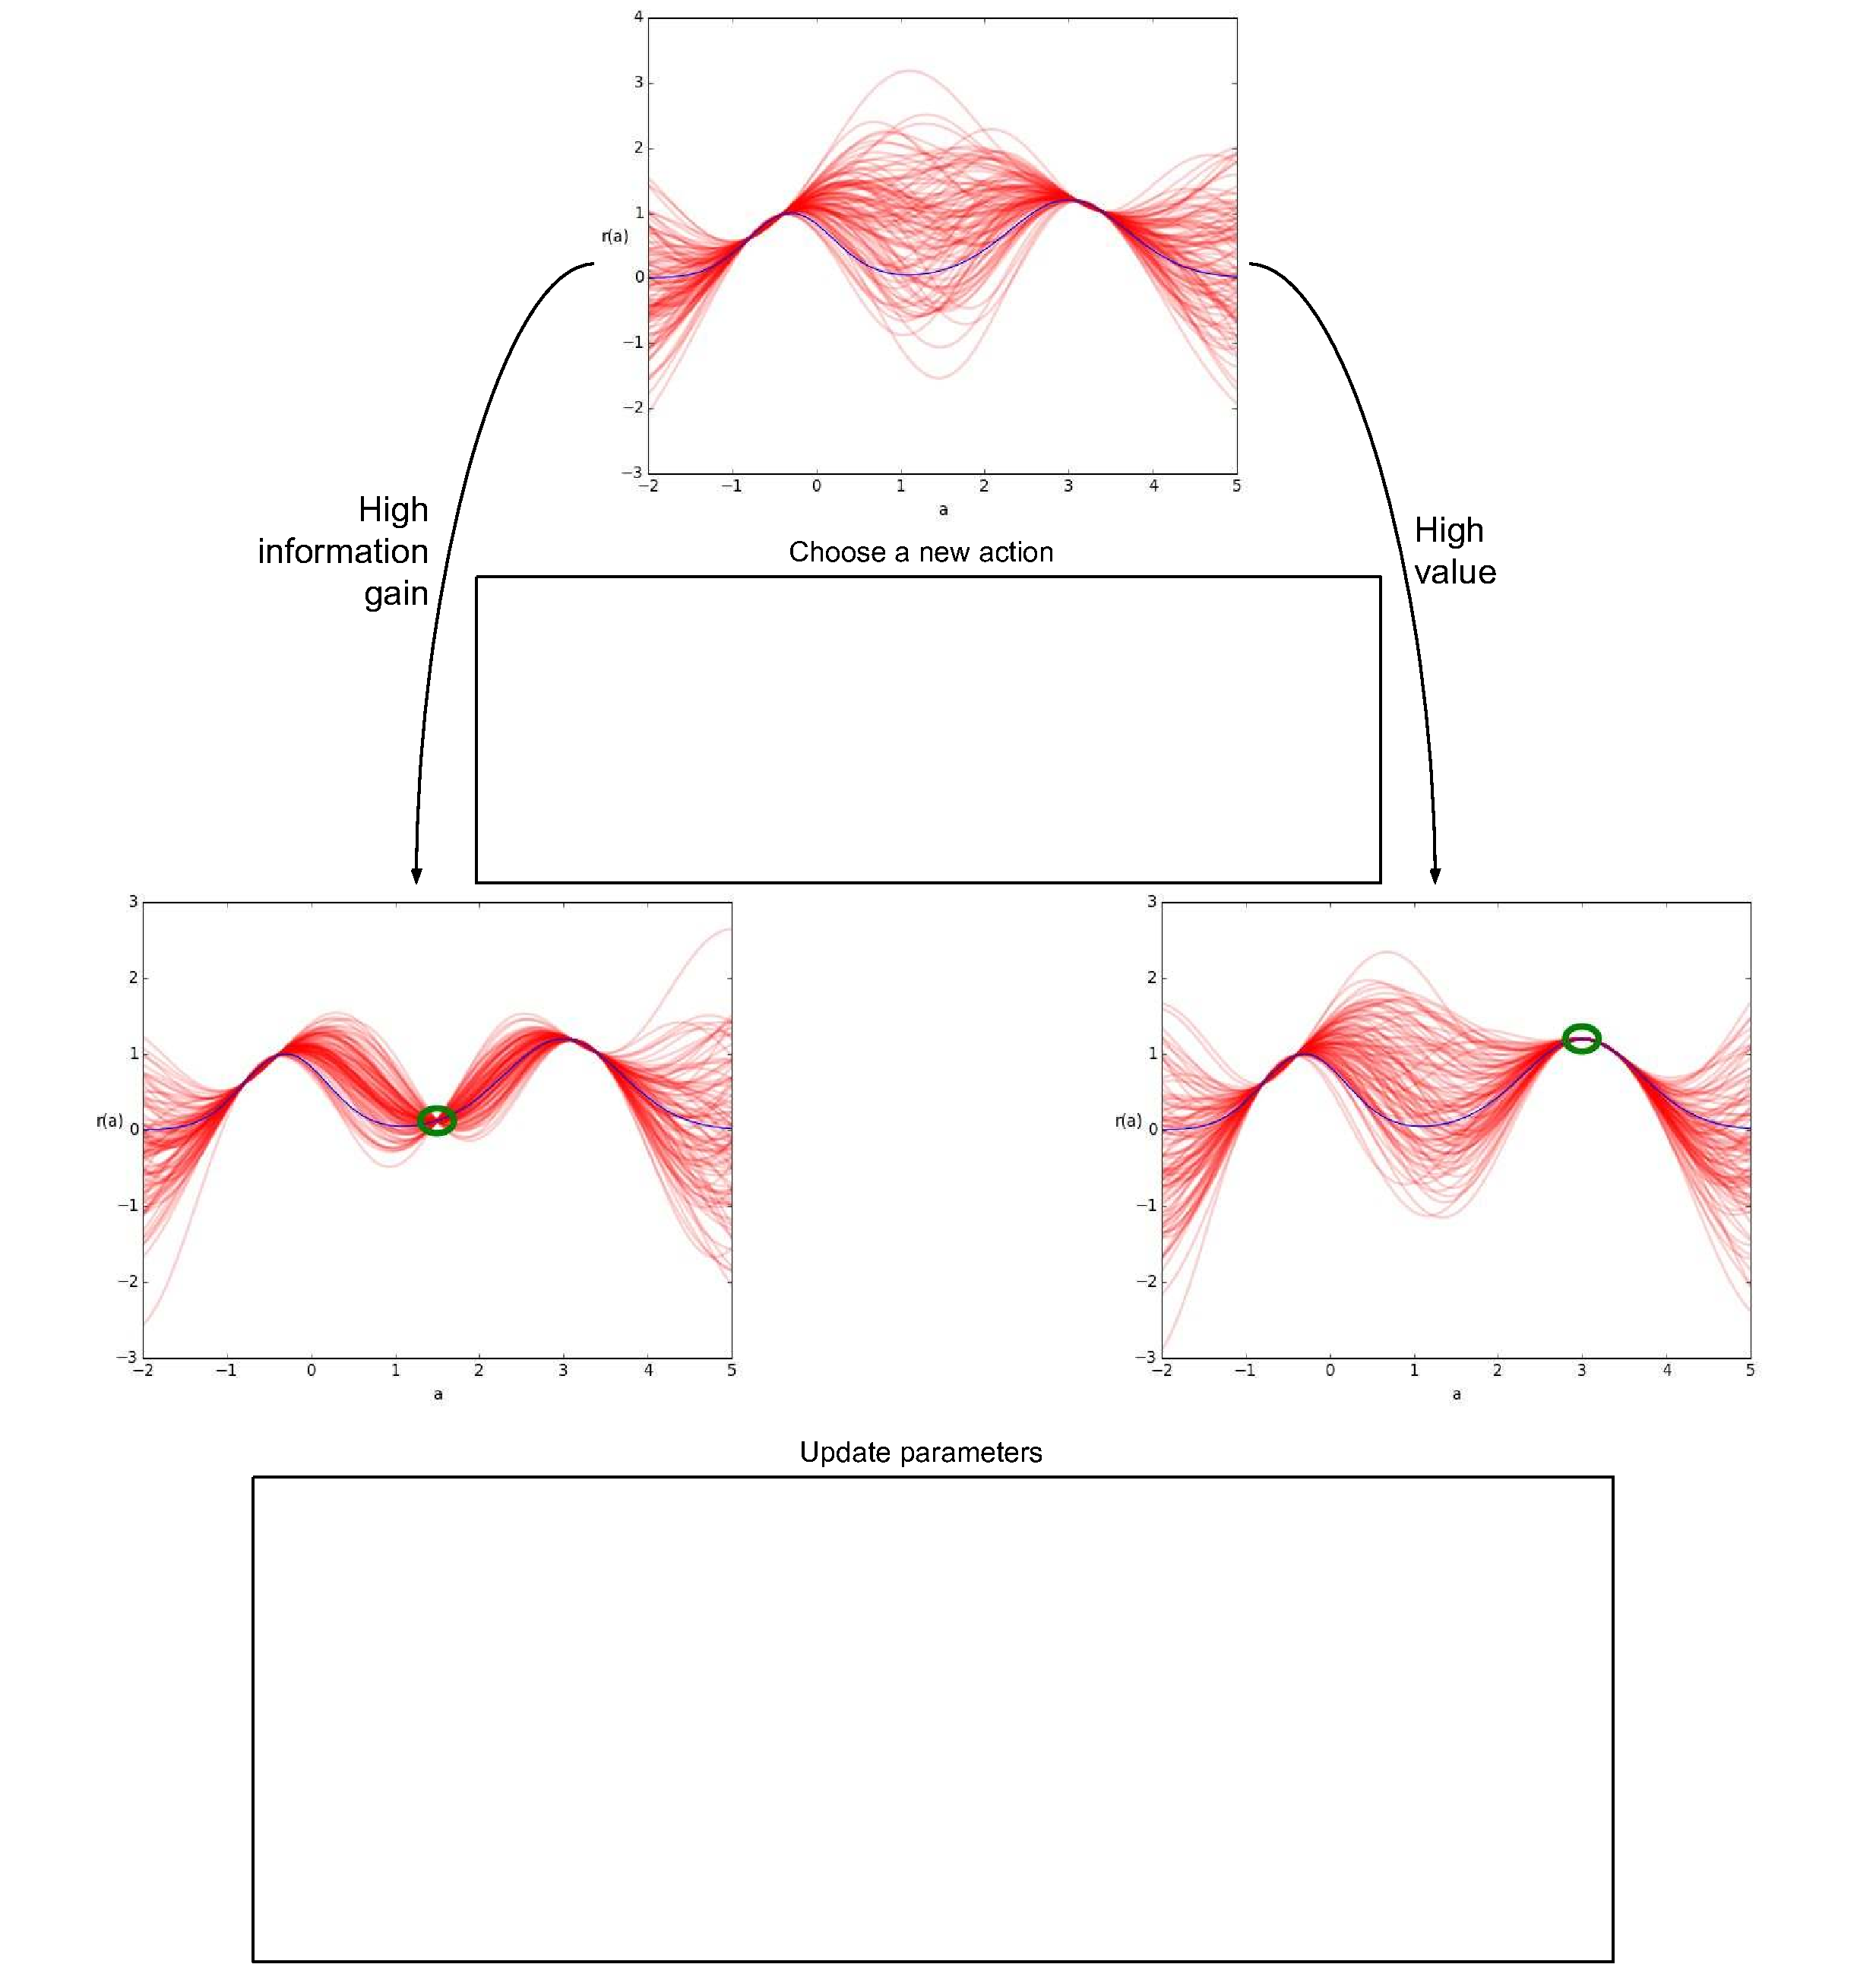
\includegraphics[width=\linewidth]{figs/slide2.pdf}
  \caption{
    Two possible actions (in green) for an iteration of Thompson sampling.  The
    believed distribution on the value function $V$ is depicted in red.  In this
    example, the true reward function is deterministic, and is drawn in blue.
    The action on the right receives a high reward, while the action on the left
    receives a low reward but greatly improves the accuracy of the believed
    distribution on $V$.  The transition operators $\tau_\search$ and
    $\tau_\update$ are described in Section \ref{sec:math-spec}.
  }
  \label{fig:slide2}
\end{figure}

Typically, when Thompson sampling is implemented, the search over contexts
$\ttheta \in \Theta$ is limited by the choice of representation.  In
traditional programming environments, $\theta$ often consists of a few
numerical parameters for a family of distributions of a fixed functional
form.  With work, a mixture of a few functional forms is possible; but
without probabilistic programming machinery, implementing a rich context
space $\Theta$ would be an unworkably large technical burden.  In a
probabilstic programing language, however, the representation of
heterogeneously structured or infinite-dimensional context spaces is quite
natural.  Any computable model of the conditional distributions
$\br{P\pn{r \mvert a}}_{a \in \Acal}$ can be represented as a stochastic
procedure $(\lambda (a) \ldots)$.  Thus, for computational Thompson sampling,
the most general context space $\widehat\Theta$ is the space of program texts.
Any other context space $\Theta$ has a natural embedding as a subset of
$\widehat\Theta$.

\subsection{Thompson Sampling with a Statistical Memoizer}
\label{sec:thompson-mem-em}
Thompson sampling as described above can be expressed compactly in terms of a
statistical memoizer, as in Listing \ref{lst:thompson-mem-em} (see also Figure
\ref{fig:slide1}).  Here and in what follows, to simplify the treatment, we
assume the true reward function is deterministic, i.e., for each fixed $a$, the
conditional distribution $P_\true\pn{r \mvert a}$ is a delta distribution.  We
thus treat the notations $a,r,\abf_\past,\rbf_\past$ as synonyms for
$x,y,\xbf_\past,\ybf_\past$, respectively, differing only in that they carry the
connotations of ``action'' and ``reward.''

\FloatBarrier
\begin{lstlisting}[frame=single,language=Venture,label=lst:thompson-mem-em,caption={
  Code template for Thompson sampling in pseudo-Venture using a statistical
  memoizer.  The choice of statistical memoizer (\texttt{mem\&em}), prior on
  semicontexts (\texttt{prior\_on\_semicontexts}), and approximation strategy
  for maximizing the emulator (\texttt{argmax}) are not included.
}]
(assume theta (tag 'theta (prior_on_semicontexts)))
(assume_list (r_probe r_emulate)
             (mem&em do_action theta))
(let loop ((a (argmax r_emulate)))
  (r_probe a)
  (inference_on 'theta)
  (loop (argmax r_emulate)))
\end{lstlisting}

\FloatBarrier

In Listing \ref{lst:thompson-mem-em}, \texttt{do\_action} is a procedure which
interfaces with the outside environment and returns the reward received.
\texttt{do\_action} is wrapped in the statistical memoizer \texttt{mem\&em},
with parameters given by the semicontext \texttt{theta} (see Setion
\ref{sec:thompson-framework}).  \texttt{theta} is given a prior distribution,
and as more actions \texttt{a} are probed, inference is performed on
\texttt{theta}, and subsequent evaluations of the emulator \texttt{r\_emulate}
are affected accordingly.  The action \texttt{a} chosen at each step is
determined by the procedure \texttt{argmax}; for purposes of Thompson sampling,
\texttt{argmax} (which takes a possibly stochastic procedure as its argument)
should be implemented so that \texttt{(argmax func)} returns an approximation to
$\argmax_{\texttt{a}} \Ebkt{\texttt{(func a)}}$.

\begin{figure}[p]
  \centering
  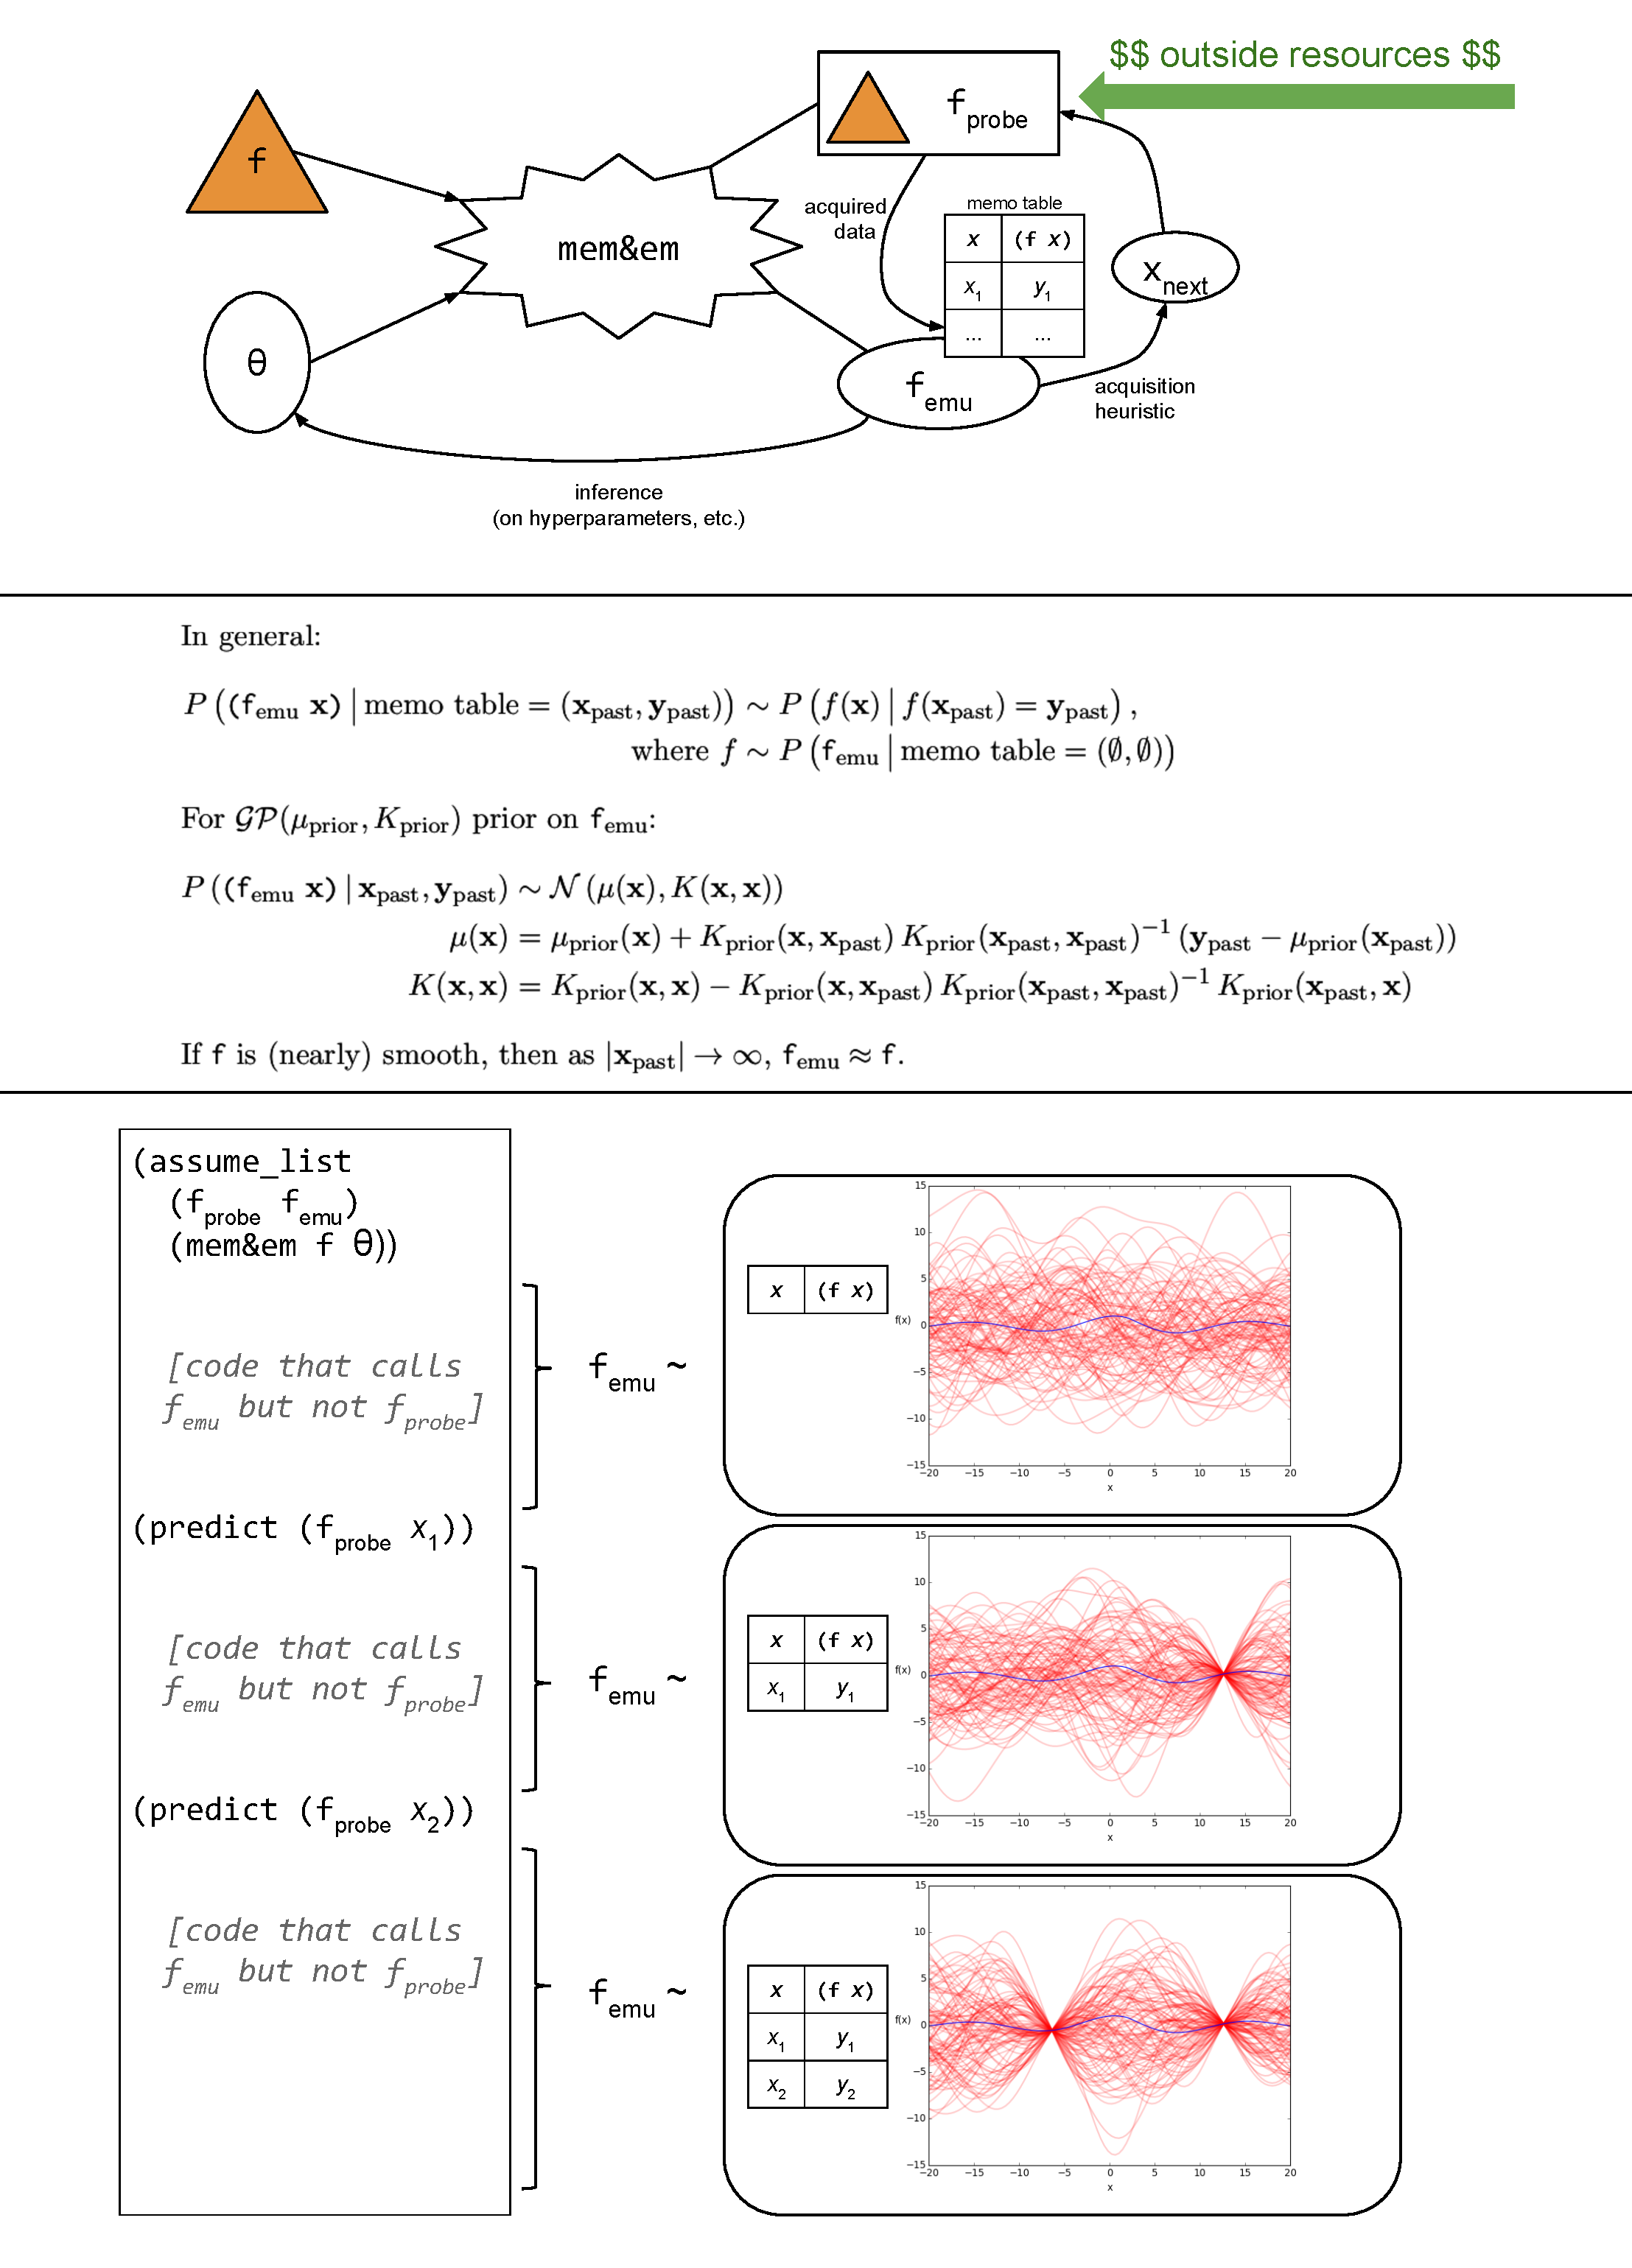
\includegraphics[height=0.8\textheight]{figs/slide1.pdf}
  \caption{
    Top: Diagrammatic representation of Thompson sampling using the statistical
    memoizer $\mm$.  The emulator $\ftt_\emu$ is used to choose a point
    $\xtt_\rmnext$ to acquire; the acquired data are incorporated into the memo
    table and the parameters $\theta$ are updated according to this new
    information.
    Middle: Mathematical specification of the statistical emulator $\ftt_\emu$.
    Bottom: Depiction of the state of the emulator after zero, one, and two
    probes have been taken.  Here the true value function $V$ is drawn in blue;
    the believed distribution on $V$ is drawn in red.  Between probes,
    $\ftt_\emu$ can be \texttt{sample}d but not \texttt{predict}ed, as its state
    (see Section \ref{sec:gps-in-pps}) must not be changed.  The state (i.e.,
    the memo table) must only be changed when $\ftt_\probe$ is called.
  }
  \label{fig:slide1}
\end{figure}

\subsection{A Mathematical Specification}\label{sec:math-spec}
Below, we give the mathematical specification of a particular application of
Thompson sampling.  This application has the following properties:
\begin{itemize}
  \item The regression function has a Gaussian process prior.
  \item The actions $a_1,a_2,\ldots \in \Acal$ are chosen by a Metropolis-like search
    strategy with Gaussian drift proposals.
  \item The hyperparameters of the Gaussian process are inferred using
    Metropolis--Hastings sampling after each action.
\end{itemize}
Details of both the model and the inference algorithm are given in the
subsections below.  An implementation will be presented in Section
\ref{sec:gp-drift}.

\subsubsection{Representations}
In this version of Thompson sampling, the contexts $\ttheta$ are Gaussian
processes over the action space $\Acal = [-20, 20] \subseteq \R$.  That is,
\[ V \sim \GP(\mu, K), \]
where the mean $\mu$ is a computable function $\Acal \to \R$ and the covariance
$K$ is a computable (symmetric, positive-semidefinite) function $\Acal \times
\Acal \to \R$.  This represents a Gaussian process $\br{R_a}_{a \in \Acal}$,
where $R_a$ represents the reward for action $a$.  Computationally, we represent
a context as a data structure
\[ \ttheta = (\theta, \abf_\past, \rbf_\past) = (\mu_\prior, K_\prior, \eta, \abf_\past, \rbf_\past), \]
where:
\begin{itemize}
  \item $\mu_\prior$ is a procedure to be used as the prior mean function.  To
    simplify the treatment, we take $\mu_\prior \equiv 0$.
  \item $K_\prior$ is a procedure to be used as the prior covariance function.
    In this example, we use a fixed functional form\footnote{
      However, within this framework there is no reason why the functional form
      of $K_\prior$ cannot itself be random and be chosen by probabilistic
      inference.  The support of $P(K_\prior)$ could, for example, be the search
      space of composite kernel structures explored in Duvenaud et
      al.~\cite{Duvenaud}.
    }
    $K_\prior = K_\prior\pn{\bullet \mvert \sigma,\ell}$, the squared exponential
    \[ K_\prior(a,a') = \sigma^2 \exp\pn{-\frac{(a-a')^2}{2\ell}}. \]
  \item $\eta$ is a set of (hyper)parameters for the mean and covariance
    functions; in this case $\eta = \br{\sigma, \ell}$.
\end{itemize}
The posterior mean and covariance for such a context $\ttheta$ are gotten by the
usual conditioning formulas (assuming, for ease of exposition as above, that the
prior mean is zero):\footnote{
  Here, for vectors $\abf = \pn{a_i}_{i=1}^{n}$ and $\abf' =
  \pn{a'_i}_{i=1}^{n'}$, $\mu(\abf)$ denotes the vector
  $\pn{\mu(a_i)}_{i=1}^{n}$ and $K(\abf,\abf')$ denotes the matrix
  $\begin{bmatrix} K(a_i, a'_j) \end{bmatrix}_{1 \leq i \leq n, 1 \leq j
  \leq n'}$.
}
\begin{align*}
  \mu(\abf)
  &= \mu\pn{\abf \mvert \abf_\past, \rbf_\past} \\
  &= K_\prior(\abf, \abf_\past)
     \,K_\prior(\abf_\past, \abf_\past)^{-1}
     \,\rbf_\past \\
  K(\abf, \abf)
  &= K\pn{\abf, \abf \mvert \abf_\past, \rbf_\past} \\
  &= K_\prior(\abf, \abf)
     - K_\prior(\abf, \abf_\past)
       \,K_\prior(\abf_\past, \abf_\past)^{-1}
       \,K_\prior(\abf_\past, \abf).
\end{align*}
Note that the context space $\Theta$ is not a finite-dimensional parametric
family, since the vectors $\abf_\past$ and $\rbf_\past$ grow as more samples are
taken.  $\Theta$ is, however, quite easily representable as a computational
procedure together with parameters and past samples, as we do in the
representation $\ttheta = (\mu_\prior, K_\prior, \eta, \abf_\past, \rbf_\past)$.

\subsubsection{Approximation Strategies}
We combine the Update and Sample steps of Algorithm \ref{alg:thompson} by
running a Metropolis--Hastings (MH) sampler whose stationary distribution is the
posterior $P\pn{\theta \mvert \abf_\past, \rbf_\past}$.  The functional forms of
$\mu_\prior$ and $K_\prior$ are fixed in our case, so inference is only done
over the parameters $\eta = \br{\sigma,\ell}$; hence we equivalently write
$P\pn{\sigma,\ell \mvert \abf_\past, \rbf_\past}$ for the stationary
distribution.  We make MH proposals to one variable at a time, using the prior
as proposal distribution:
\[
  Q_\proposal\pn{\sigma',\ell \mvert \sigma,\ell} = P(\sigma')
\]
and
\[
  Q_\proposal\pn{\sigma,\ell' \mvert \sigma,\ell} = P(\ell').
\]
The MH acceptance probability for such a proposal is
\[
  P_\accept\pn{\sigma',\ell' \mvert \sigma,\ell}
  =
  \min\br{1,\ \frac{
    Q_\proposal\pn{\sigma,\ell \mvert \sigma',\ell'}
    }{
    Q_\proposal\pn{\sigma',\ell' \mvert \sigma,\ell}
    }
  \cdot
  \frac{
    P\pn{\abf_\past,\rbf_\past \mvert \sigma',\ell'}
    }{
    P\pn{\abf_\past,\rbf_\past \mvert \sigma,\ell}
    }}
\]
Because the priors on $\sigma$ and $\ell$ are uniform in our case, the term
involving $Q_\proposal$ equals $1$ and we have simply
\begin{align*}
  P_\accept\pn{\sigma',\ell' \mvert \sigma,\ell}
  &=
  \min\br{1,\ \frac{
    P\pn{\abf_\past,\rbf_\past \mvert \sigma',\ell'}
    }{
    P\pn{\abf_\past,\rbf_\past \mvert \sigma,\ell}
    }} \\[2mm]
  &=
  \min\bigg\{1,\ \exp\bigg( -\frac12\bigg(
    \rbf_\past^T K_\prior\pn{\abf_\past, \abf_\past \mvert \sigma', \ell'}^{-1} \rbf_\past \\
  & \qquad\qquad\qquad\qquad\qquad -
    \rbf_\past^T K_\prior\pn{\abf_\past, \abf_\past \mvert \sigma, \ell}^{-1} \rbf_\past
  \bigg)\bigg)\bigg\}.
\end{align*}
The proposal and acceptance/rejection process described above define a
transition operator $\tau_\update$ which is iterated a specified number of
times; the resulting state of the MH Markov chain is taken as the sampled
semicontext $\theta$ in Step \ref{itm:thompson-step-sample} of Algorithm
\ref{alg:thompson}.

For Step \ref{itm:thompson-step-search} (Search) of Thompson sampling, we
explore the action space using an MH-like transition operator $\tau_\search$.
As in MH, each iteration of $\tau_\search$ produces a proposal which is either
accepted or rejected, and the state of this Markov chain after a specified
number of steps is the new action $a$.  The Markov chain's initial state is the
most recent action, and the proposal distribution is Gaussian drift:
\[ Q_\proposal\pn{a' \mvert a} \sim \Ncal(a,\,\propstd^2), \]
where the drift width $\propstd$ is specified ahead of time.  The acceptance
probability of such a proposal is
\[ P_\accept\pn{a' \mvert a} = \min\br{1,\ \exp\pn{-E\pn{a' \mvert a}}}, \]
where the energy function $E\pn{\bullet \mvert a}$ is given by a Monte Carlo
estimate of the difference in value from the current action:
\[ E\pn{a' \mvert a} = -\frac1s \pn{\muhat(a') - \muhat(a)} \]
where
\[ \muhat(a) = \frac{1}{N_\avg} \sum_{i=1}^{N_\avg} \widetilde{r}_{i,a} \]
and
\[ \widetilde{r}_{i,a} \sim \Ncal(\mu(a), K(a,a)) \]
and $\br{\widetilde{r}_{i,a}}_{i=1}^{N_\avg}$ are i.i.d.\ for a fixed $a$.
Here the temperature parameter $s \geq 0$ and the population size $N_\avg$ are
specified ahead of time.  Note the following properties of the above acceptance
probability:
\begin{itemize}
  \item Proposals of estimated value higher than that of the current action are
    always accepted, while proposals of estimated value lower than that of the
    current action are accepted with a probability that decays exponentially
    with respect to the difference in value.
  \item The rate of the decay is determined by the temperature parameter $s$,
    where high temperature corresponds to generous acceptance probabilities.
    For $s=0$, all proposals of lower value are rejected; for $s=\infty$, all
    proposals are accepted.
  \item For points $a$ at which the posterior mean $\mu(a)$ is low but the
    posterior variance $K(a,a)$ is high, it is possible (especially when
    $N_\avg$ is small) to draw a ``wild'' value of $\muhat(a)$, resulting in a
    favorable acceptance probability.
\end{itemize}
Indeed, taking an action $a$ with low estimated value but high uncertainty
serves the useful function of improving the accuracy of the estimated value
function at points near $a$ (see Figure \ref{fig:slide2}).\footnote{
  At least, this is true when we use a smoothing prior covariance function such
  as the squared exponential.
}$^,$\footnote{
  For this reason, we consider the sensitivity of $\muhat$ to uncertainty to be
  a desirable property; indeed, this is why we use $\muhat$ rather than the
  exact posterior mean $\mu$.
}
